\documentclass[a4paper]{report}

\usepackage{anysize}
\usepackage[english]{babel}
\usepackage{comment}
\usepackage{paralist}
\usepackage{hyperref}
\usepackage[pdftex]{graphicx}
\usepackage{applekeys}

\marginsize{2.5cm}{2.5cm}{2cm}{2cm}

\newcommand{\blankline}{\par\vspace{5mm}}
\newcommand{\tab}{\hspace*{2em}}


\begin{document}
	
\begin{center}
	\textsc{\Large Project Big Data}
	\blankline
	{\large Syllabus}
\end{center}

\section*{Organizational}

\paragraph{Course information}
This course aims to integrate various aspects involved with data science and to teach the fundamentals of working with big data (including an
introduction to Hadoop). Topics include visualization of data; preparing data for processing (machine learning or data mining); storing unstructured data; and scaling techniques for working with big volumes of data. Python is used throughout this hands-on course.

\paragraph{Staff}
The organizers for this course are:
\begin{itemize}
	\setlength\itemsep{0mm}
	\item Irving van Heuven van Staereling (\texttt{i.i.van.heuvenvanstaereling@vu.nl})
	\item Rutger Hofman (\texttt{r.f.h.hofman@vu.nl})
	\item Nanne Dieleman (\texttt{n.a.dieleman@vu.nl})
\end{itemize}
For questions that cannot be answered during the working group, contact \texttt{pbd-vu@gmail.com}, which sends an email to all instructors. Any of the instructors will try to reply as soon as possible.

\paragraph{Format}
The entire course is done in groups of two students. You should select your own partner. There is an one-time opportunity to switch partners after the first week.

At the end of the fourth week each group is expected to give a 10 - 12 minute presentation. The presentations are grouped in slots of one hour each. All three groups that present in a slot should be present during the entire hour. Be prepared by arriving on time and having your presentation ready in pdf format on a usb-stick and online.

As for the style of your slides, make sure they look professional, have good contrast, are readable from the back, and have the same style as your partner's. Practice with your partner to ensure a smooth transition between you two and to stick to the time limit. After 10 minutes we will give a sign. Avoid hitting the 12 minute mark because we will terminate your presentation to give the audience the opportunity to ask questions.

You are expected to be (or seem) interested in the presentations and discussions of fellow students. Asking insightful questions is encouraged, while being a distraction will negatively affect your grade.

\paragraph{Literature}
The powerpoint slides cover all materials for this course.

\paragraph{Schedule}
All relevant dates are summarized in the table below.

\begin{table}[h!]
	\begin{tabular}{| l | l | l | l | l | l |}
		\hline
		\textbf{Day}	&	\textbf{Date}	& \textbf{Time}	& \textbf{Type}			& \textbf{Location}	& \textbf{Instructors}	\\
		\hline
		Monday			&	04-06			& 11:00 - 12:45	& Lecture				& WN-C121			& Irving				\\
		Tuesday			&	05-06			& 10:00 - 12:45	& Working group			& HG-06A33			& Irving, Nanne, Rutger	\\
		Thursday		&	07-06			& 10:00 - 12:45	& Working group			& WN-C121			& Irving, Nanne, Rutger	\\
		\hline
		Monday			&	11-06			& 11:00 - 12:45	& Lecture				& WN-C121			& Irving				\\
		Tuesday			&	12-06			& 10:00 - 12:45	& Working group			& HG-06A33			& Irving, Nanne, Rutger	\\
		Thursday		&	14-06			& 10:00 - 12:45	& Working group			& WN-C121			& Irving, Nanne, Rutger	\\
		\hline
		Monday			&	18-06			& 11:00 - 12:45	& Lecture				& WN-C121			& Irving				\\
		Tuesday			&	19-06			& 10:00 - 12:45	& Working group			& HG-06A33			& Irving, Rutger	\\
		Thursday		&	21-06			& 10:00 - 12:45	& Working group			& WN-C121			& Irving, Rutger	\\
		\hline
		Tuesday			&	26-06			& 10:00 - 12:45	& Working group			& HG-02A33			& Irving, Rutger	\\
		Thursday		&	28-06			& 09:00 - 12:45	& Presentations			& WN-S624/WN-S664	& Irving, Rutger	\\
		\hline
	\end{tabular}
\end{table}

\paragraph{Attendance}
Attendance is only mandatory for the presentations.

\paragraph{Grading}
The tasks for the course (including weights) are summarized in the table below.

\begin{table}[h!]
	\begin{tabular}{| l | l | l |}
		\hline
		\textbf{Assignment} & \textbf{Weight}	& \textbf{Deadline}					\\
		\hline
		Week 1				&	15\%			& Friday, June 8, 23:59				\\
		\hline
		Week 2				&	15\%			& Friday, June 15, 23:59			\\
		\hline
		Week 3				&	15\%			& Friday, June 22, 23:59			\\
		\hline
		Presentation		&	20\%			& Thursday, June 28, 09:00 - 12:45	\\
		\hline
		Report				&	35\%			& Friday, June 29, 23:59			\\
		\hline
	\end{tabular}
\end{table}
The criteria for the report and presentation are included at the end of this syllabus. Grades for each part are given in the range 1--10, even for missing work. You pass if the weighted average is above 5.5. In principle, both group members get the same grade, except for the presentation.

\paragraph{If you took this course in a previous year}
If you took this course in a previous year and finished part of the assignments, you cannot do those parts with someone else this year. For those assignments you either have to work with the same partner as last year, or by yourself.

If, in a previous year, you received a grade for the assignment of week 1, you either have to do this year's command line assignment or this year's complete assignment. If you only do the command line assignment, the grade will be weighted with your previous grade.

If, in a previous year, you received a grade for any other assignment, report or presentation, you can keep that grade by not handing in a new solution or report or not giving a new presentation. If you choose to do this, please inform the course coordinator about your choice.

If you were graded for any part in a previous year and hand in a new solution, only the last grade counts.

\paragraph{Plagiarism}
The assignments and grading schemes have been designed for groups of two. Collaborating with other groups is not permitted. Using the internet as a passive resource is allowed. That means that you can search for solutions and copy code, as long as you indicate which parts have been copied and from where. Asking questions online is not permitted. All your code will be scanned for plagiarism. Violations are always reported to the Board of Examiners and may result in disciplinary measures.

\blankline

\section*{Software}
You will use Python, MongoDB and command line tools. Installation instructions for Windows and Mac OS X are included in this syllabus.

\subsection*{Windows}
\paragraph{Command line tools}
The command line on Windows is traditionally not well developed (we will
ignore PowerShell in this course). Fortunately, many tools from *nix
have been ported to Windows. One of these ports is \mbox{unxutils}
(\url{https://sourceforge.net/projects/unxutils/}). After downloading
and opening the zip file, you find all useful tools in
\textit{usr{\textbackslash}local{\textbackslash}wbin}. Copy the files,
then paste them into a new folder \textit{C:{\textbackslash}Program~Files{\textbackslash}unxutils}.

\noindent\begin{center}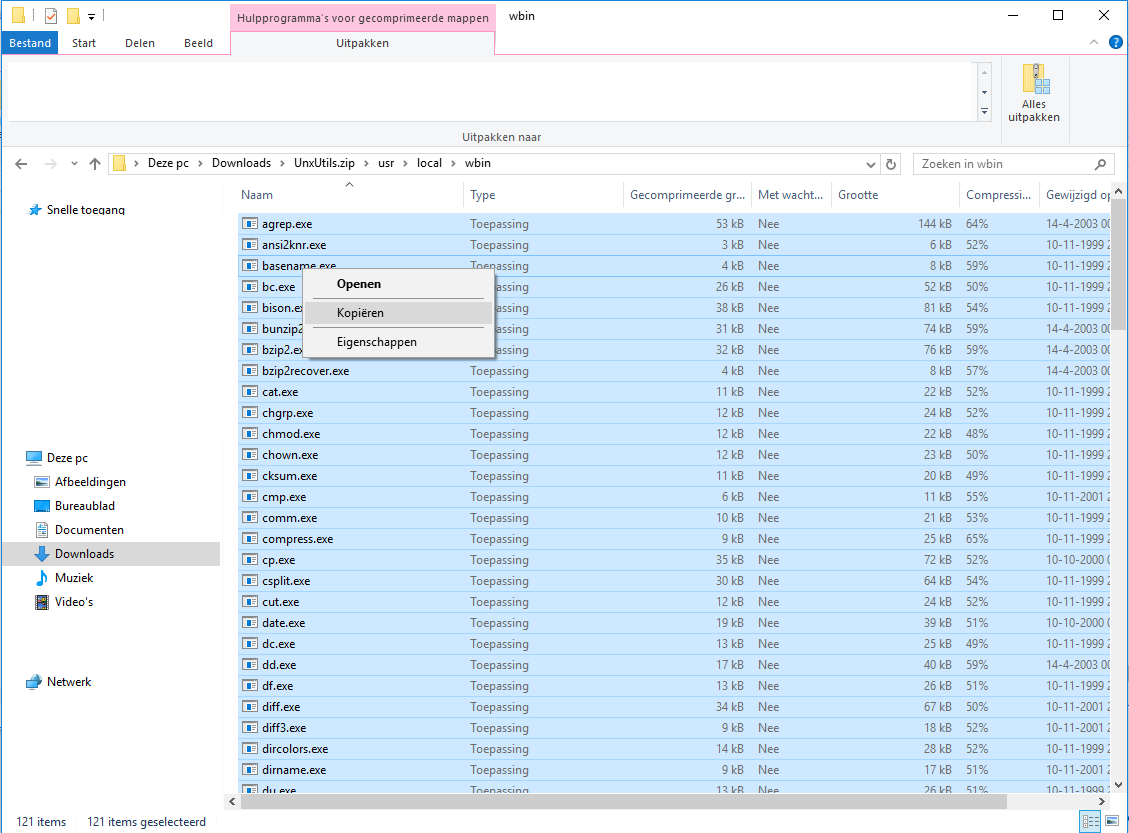
\includegraphics[width=5.552in,height=4.098in]{Syllabus-img1.png}\end{center}

Next, add the folder \textit{C:{\textbackslash}Program
Files{\textbackslash}unxutils} to the path, so Windows knows where the
commands are located. To do this, press winkey+pause, go to advanced
system settings, and then to \textit{environment variables} (Dutch:
\textit{omgevingsvariabelen}) in the \textit{advanced} tab.

\noindent\begin{center}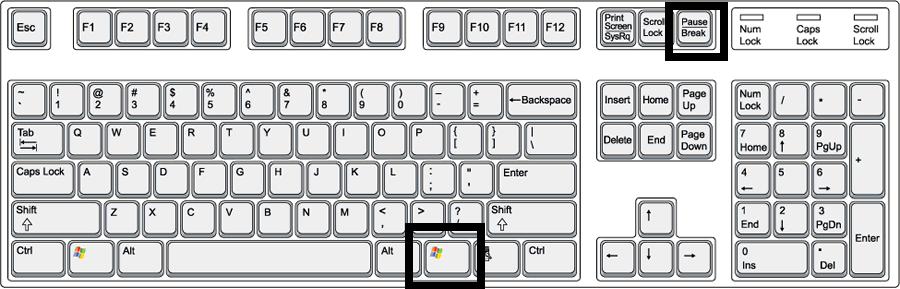
\includegraphics[width=6.5in,height=2.0846in]{Syllabus-img2.png}
\end{center}

\noindent\begin{center}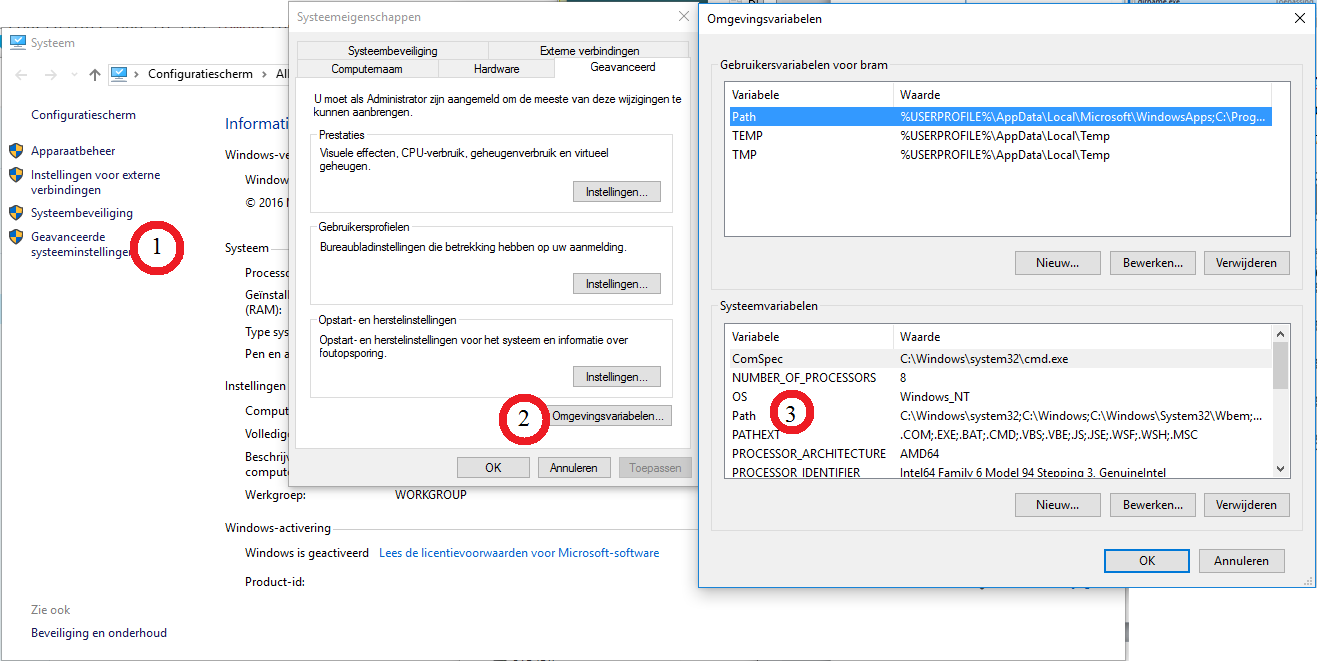
\includegraphics[width=6.4866in,height=3.2535in]{Syllabus-img3.png}
\end{center}

Add the folder \textit{C:{\textbackslash}Program~Files{\textbackslash}unxutils}
to the system path. In earlier versions
of Windows the path is a single text field where you can add the new
folder at the end, separating it with a semicolon (;). In newer
versions of Windows adding an entry to the path is straightforward.

Some tools already exist in Windows but have a different implementation,
such as sort. Rename sort.exe to sort2.exe to make it available.
Don{\textquoteright}t forget to enter sort2 instead of sort whenever
you want to run sort.

To verify if the install is successful, open the command prompt (hit the
winkey, type {\small\texttt{cmd}} and hit return) and type
{\textquoteleft}grep{\textquoteright}. If it shows
{\textquotedblleft}Usage: grep [OPTION]{\textquotedblright} the install
is complete. If it says
{\textquotedblleft}{\textquoteright}grep{\textquoteright} is not
recognized{\textquotedblright} the install is incomplete. Enter the
command {\small\texttt{path}} to see if the path is correct.

\paragraph{Python}
Any Python 3 distribution with pandas, numpy, pymongo, re, sklearn and
matplotlib will do. We recommend WinPython
(\url{https://winpython.github.io/}). Select the latest release and the
latest subrelease, in this case 3.6.1, and click
{\textquotedblleft}Downloads{\textquotedblright}. 

\noindent\begin{center}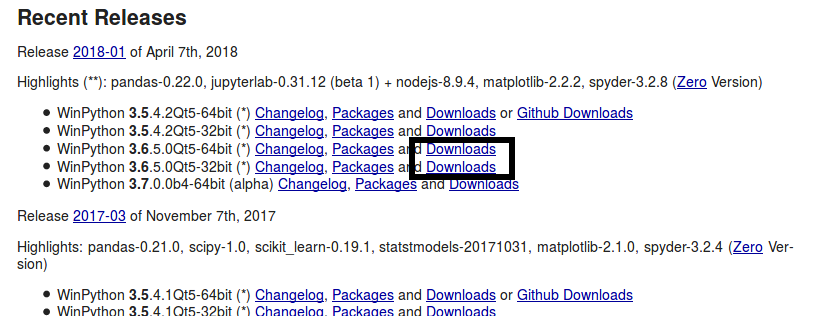
\includegraphics[width=6.4925in,height=2.3134in]{Syllabus-download-WinPython.png}
\end{center}

To determine if you need the 32bit or 64bit version, press winkey+pause
(see the install instructions for command line tools) and look for
{\textquotedblleft}system type{\textquotedblright}. Make sure to
download the full version (which is around 300 MB) and not the Zero
version (around 25 MB).

After downloading, run the .exe file and install WinPython to any
folder, but be aware that a path containing spaces may result in
unexpected behavior.

Now open the folder WinPython was installed to and run
\textit{Spyder.exe}. If you need to install extra modules, run
\textit{WinPython Command Prompt.exe} and use {\small\texttt{pip install}}.

\paragraph{MongoDB}
MongoDB can be downloaded from
\url{https://www.mongodb.com/download-center}; use the pane labeled
``Community Center''. The version that is
selected runs on both the 32 bit and the 64 bit version of Windows 7
and above. Run the installation wizard. Installation under Windows-10 may be
a bit problematic. If you run into the error ``setup wizard ended
prematurely'', uncheck the ``Install MongoDB Compass'' checkbox, somewhere in
the setup process. After successful installation, create the folder
\textit{C:{\textbackslash}data{\textbackslash}db}. Then go to
\textit{C:{\textbackslash}Program
Files{\textbackslash}MongoDB{\textbackslash}Server{\textbackslash}3.4{\textbackslash}bin}
and run \textit{mongod.exe}. The following window should appear,
indicating that MongoDB is running:

\noindent\begin{center}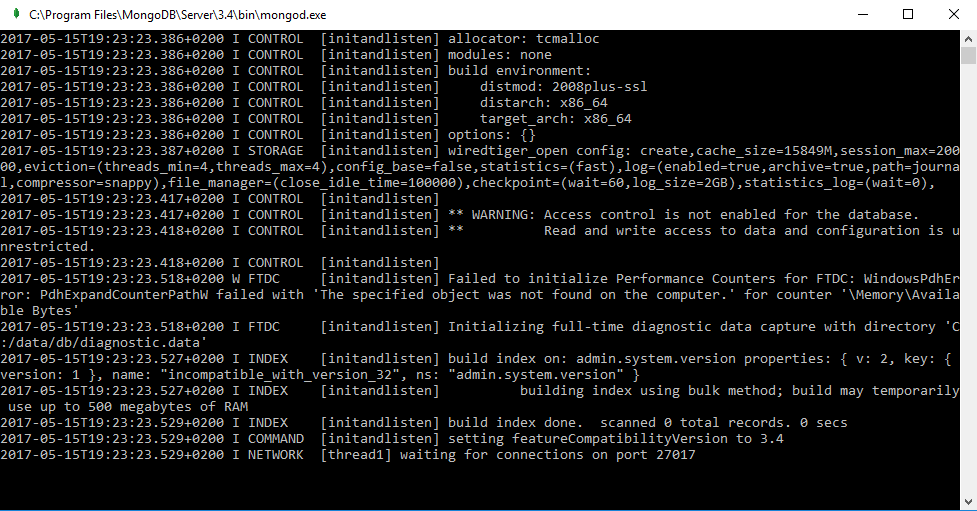
\includegraphics[width=6.4925in,height=3.3957in]{Syllabus-img5.png}
\end{center}

If the window closes directly by itself, run \textit{mongod.exe} from
the command line to see an error message.

\subsection*{Mac OS X}

\paragraph{Command line tools}
Mac OS X already has all necessary tools, except gawk. You can open the
terminal by going into Spotlight (with command (\cmdkey) space, or by
clicking on the magnifying glass in the top right corner of your
screen) and searching for and selecting Terminal. 

Install homebrew by copy-pasting the following command into the
Terminal:

\noindent{\small\texttt{
/usr/bin/ruby -e \$(curl -fsSL https://raw.githubusercontent.com/Homebrew/install/master/install)}}

brew is installed into {\small\texttt{/usr/local/bin}}. Likewise,
brew uses {\small\texttt{/usr/local/bin}} to install other software
into. To use brew and software installed by brew, you need to add
{\small\texttt{/usr/local/bin}} to your {\small\texttt{PATH}} environment
variable as follows. Edit {\small\texttt{\textasciitilde/.bashrc}}
and add the following line:

\noindent{\small\texttt{export PATH=\$PATH:/usr/local/bin}}

Save. Then close and reopen your Terminal. When you type
the command {\small\texttt{which brew}} it should report:
{\small\texttt{/usr/local/bin/brew}}

Once homebrew is successfully installed on your system, install gawk via the
command {\small\texttt{brew install gawk}}. Verify that gawk is found and
gives sane output by typing {\small\texttt{gawk --help}} to the Terminal.

\paragraph{Python}
Download the .pkg installer for Python 3.6.5 here:

\url{https://www.python.org/ftp/python/3.6.5/python-3.6.5-macosx10.6.pkg}

Run the installer by executing the .pkg, and install Python by following
the instructions.

\paragraph{MongoDB}
MongoDB can be downloaded from
\url{https://www.mongodb.com/download-center}; use the pane labeled
``Community Server''. Click OSX, download and
extract the .tgz file to any folder. In the terminal, go to that folder
and create a subfolder {\small\texttt{data/db}} with the command {\small\texttt{mkdir
-p data/dp}} to complete the install. Each time you{\textquoteright}d
like to use MongoDB, open the terminal, go to the right folder, and run
{\small\texttt{bin/mongod -{}-dpath data/db}}.

Alternatively, MongoDB can be installed with the command {\small\texttt{brew
install mongodb -{}-with-openssl}}. Subsequently, create a mongodb data
directory in your home directory with the command {\small\texttt{mkdir -p
\~{}/data/dp}}. Running the command {\small\texttt{bin/mongod -{}-dpath
\~{}/data/db}} should show you the following message:

\noindent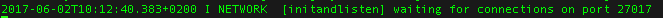
\includegraphics[width=6.4953in,height=0.1783in]{Syllabus-img6.png} 

\paragraph{Spyder editor}
Python comes with a package manager called {\small\texttt{pip}} (sometimes also
called {\small\texttt{pip-3.5}} or {\small\texttt{pip-3.6}}; replace the following commands with
the name that works on your system). To install the Spyder editor,
type the following two commands into the Terminal: 

\noindent{\small\texttt{pip install PyQt5}}
\\
{\small\texttt{pip install spyder}}

\paragraph{Python packages}
In a similar way, use {\small\texttt{pip install {\textless}packagename{\textgreater}}} to install the following packages: pandas, numpy, pymongo, re, sklearn and matplotlib 

\blankline

\section*{Criteria for final report and presentation}

\paragraph{Criteria for final report}

\begin{enumerate}
	\item Quality of written text (10\%)
	\begin{compactitem}
		\item The text is free from grammatical errors and spelling mistakes
		\item The text has a clear and logical structure
	\end{compactitem}
	\item Quality of data analyses (40\%)
	\begin{compactitem}
		\item Python code is complete and correct (see individual assignments for the credits that can be earned per component)
		\item The reported descriptive statistics are complete (for example, not just the mean, but also the standard deviation)
		\item Assumptions for statistical tests have been checked
		\item The appropriate statistical tests have been applied. When there is doubt, the choice is motivated.
	\end{compactitem}
	\item Quality of the visualizations (20\%)
	\begin{compactitem}
		\item All graphs have descriptive labels on their axes
		\item The values on the axes have units
		\item The intervals of the values on the axes are suitable
		\item The graph is clear and legible, and uses an appropriate font size
		\item When appropriate, graphs contain a legible and clear legend
		\item The use of color in the graphs is helpful for understanding the graphs
	\end{compactitem}
	\item Quality of the interpretations of the analyses (20\%)
	\begin{compactitem}
		\item Interpretations are appropriately nuanced
		\item Interpretations are adequately motivated
		\item Alternative interpretations are discussed
	\end{compactitem}
	\item Formal requirements (10\%)
	\begin{compactitem}
		\item The report should be handed in as a PDF document
		\item Both the Python file and the final report have the correct filenames
		\item The report contains a cover page that includes the names and student numbers of the authors, the name of the course, and the date on which the report was handed in
		\item The report contains page numbers in the bottom right corner
	\end{compactitem}
\end{enumerate}

\paragraph{Criteria for the presentation}

\begin{enumerate}
	\item Quality of the content (60\%)
	\begin{compactitem}
		\item The presentation contains a clear research statement.
		\item The presentation is focused and to the point. It is tailored towards its target audience (students Business Analytics before they take Project Big Data).
		\item Through the presentation, it becomes clear what the motivation for the research statement is.
		\item The presentation contains visualizations of the data that support the main narrative of the presentation. These visualizations should be made with the presentation (projector, etc.) in mind.
		\item The presentation has a clear and transparent structure.
		\item The presentation offers relevant points for discussion on the basis of the performed analyses.
	\end{compactitem}
	\item Presentation skills (30\%)
	\begin{compactitem}
		\item The speaker speaks clearly, audibly, and with good pace.
		\item The speaker keeps everyone in the audience engaged (eye contact, etc.).
		\item The speaker uses his or her hands for non-verbal communication.
		\item The speaker uses body language to convey confidence.
		\item The speaker stays within the allotted time.
		\item The speaker responds to questions adequately.
	\end{compactitem}
	\item Formal requirements (10\%)
	\begin{compactitem}
		\item The presentation is accompanied with a slide deck. The first slide contains the title of the presentation, the speakers' names, the date, and the title of the course.
		\item The slides contain sources where appropriate (e.g., citations, borrowed figures, etc.)
	\end{compactitem}
\end{enumerate}


\end{document}
